
\begin{figure}[H]
			\centering		
			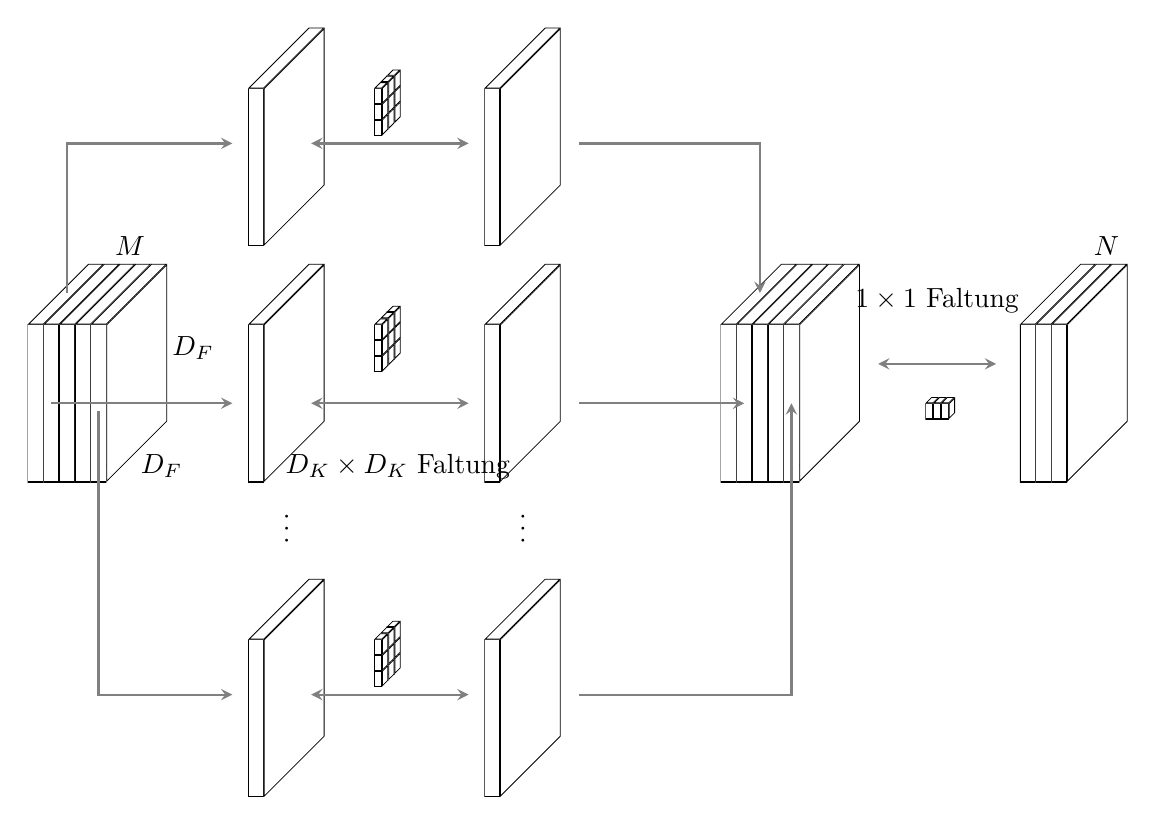
\begin{tikzpicture}
				\pgfmathsetmacro{\cubex}{0.2}
				\pgfmathsetmacro{\cubey}{2}
				\pgfmathsetmacro{\cubez}{2}
				
				\begin{scope}[yshift=-2cm,line width=0.2mm]
				\begin{scope}
				\clip[] (-0.8,0,0) -- ++(-\cubex,0,0) -- ++(0,-\cubey,0) -- ++(\cubex,0,0) -- cycle;
				\draw[fill=white] (-0.8,0,0) -- ++(-\cubex,0,0) -- ++(0,-\cubey,0) -- ++(\cubex,0,0) -- cycle;
				\end{scope}
				\begin{scope}
				\clip[] (-0.8,0,0) -- ++(0,0,-\cubez) -- ++(0,-\cubey,0) -- ++(0,0,\cubez) -- cycle;
				\draw[fill=white] (-0.8,0,0) -- ++(0,0,-\cubez) -- ++(0,-\cubey,0) -- ++(0,0,\cubez) -- cycle;
				\end{scope}
				\begin{scope}
				\clip[] (-0.8,0,0) -- ++(-\cubex,0,0) -- ++(0,0,-\cubez) -- ++(\cubex,0,0) -- cycle;
				\draw[fill=white] (-0.8,0,0) -- ++(-\cubex,0,0) -- ++(0,0,-\cubez) -- ++(\cubex,0,0) -- cycle;
				\end{scope}
				
				\begin{scope}
				\clip[] (-0.6,0,0) -- ++(-\cubex,0,0) -- ++(0,-\cubey,0) -- ++(\cubex,0,0) -- cycle;
				\draw[fill=white] (-0.6,0,0) -- ++(-\cubex,0,0) -- ++(0,-\cubey,0) -- ++(\cubex,0,0) -- cycle;
				\end{scope}
				\begin{scope}
				\clip[] (-0.6,0,0) -- ++(0,0,-\cubez) -- ++(0,-\cubey,0) -- ++(0,0,\cubez) -- cycle;
				\draw[fill=white] (-0.6,0,0) -- ++(0,0,-\cubez) -- ++(0,-\cubey,0) -- ++(0,0,\cubez) -- cycle;
				\end{scope}
				\begin{scope}
				\clip[] (-0.6,0,0) -- ++(-\cubex,0,0) -- ++(0,0,-\cubez) -- ++(\cubex,0,0) -- cycle;
				\draw[fill=white] (-0.6,0,0) -- ++(-\cubex,0,0) -- ++(0,0,-\cubez) -- ++(\cubex,0,0) -- cycle;
				\end{scope}
				
				\begin{scope}
				\clip[] (-0.4,0,0) -- ++(-\cubex,0,0) -- ++(0,-\cubey,0) -- ++(\cubex,0,0) -- cycle;
				\draw[fill=white] (-0.4,0,0) -- ++(-\cubex,0,0) -- ++(0,-\cubey,0) -- ++(\cubex,0,0) -- cycle;
				\end{scope}
				\begin{scope}
				\clip[] (-0.4,0,0) -- ++(0,0,-\cubez) -- ++(0,-\cubey,0) -- ++(0,0,\cubez) -- cycle;
				\draw[fill=white] (-0.4,0,0) -- ++(0,0,-\cubez) -- ++(0,-\cubey,0) -- ++(0,0,\cubez) -- cycle;
				\end{scope}
				\begin{scope}
				\clip[] (-0.4,0,0) -- ++(-\cubex,0,0) -- ++(0,0,-\cubez) -- ++(\cubex,0,0) -- cycle;
				\draw[fill=white] (-0.4,0,0) -- ++(-\cubex,0,0) -- ++(0,0,-\cubez) -- ++(\cubex,0,0) -- cycle;
				\end{scope}
				
				\begin{scope}
				\clip[] (-0.2,0,0) -- ++(-\cubex,0,0) -- ++(0,-\cubey,0) -- ++(\cubex,0,0) -- cycle;
				\draw[fill=white] (-0.2,0,0) -- ++(-\cubex,0,0) -- ++(0,-\cubey,0) -- ++(\cubex,0,0) -- cycle;
				\end{scope}
				\begin{scope}
				\clip[] (-0.2,0,0) -- ++(0,0,-\cubez) -- ++(0,-\cubey,0) -- ++(0,0,\cubez) -- cycle;
				\draw[fill=white] (-0.2,0,0) -- ++(0,0,-\cubez) -- ++(0,-\cubey,0) -- ++(0,0,\cubez) -- cycle;
				\end{scope}
				\begin{scope}
				\clip[] (-0.2,0,0) -- ++(-\cubex,0,0) -- ++(0,0,-\cubez) -- ++(\cubex,0,0) -- cycle;
				\draw[fill=white] (-0.2,0,0) -- ++(-\cubex,0,0) -- ++(0,0,-\cubez) -- ++(\cubex,0,0) -- cycle;
				\end{scope}
				
				\begin{scope}
				\clip[] (0,0,0) -- ++(-\cubex,0,0) -- ++(0,-\cubey,0) -- ++(\cubex,0,0) -- cycle;
				\draw[fill=white] (0,0,0) -- ++(-\cubex,0,0) -- ++(0,-\cubey,0) -- ++(\cubex,0,0) -- cycle;
				\end{scope}
				\begin{scope}
				\clip[] (0,0,0) -- ++(0,0,-\cubez) -- ++(0,-\cubey,0) -- ++(0,0,\cubez) -- cycle;
				\draw[fill=white] (0,0,0) -- ++(0,0,-\cubez) -- ++(0,-\cubey,0) -- ++(0,0,\cubez) -- cycle;
				\end{scope}
				\begin{scope}
				\clip[] (0,0,0) -- ++(-\cubex,0,0) -- ++(0,0,-\cubez) -- ++(\cubex,0,0) -- cycle;
				\draw[fill=white] (0,0,0) -- ++(-\cubex,0,0) -- ++(0,0,-\cubez) -- ++(\cubex,0,0) -- cycle;
				\end{scope}
				
				\begin{scope}
				\clip[] (2,3,0) -- ++(-\cubex,0,0) -- ++(0,-\cubey,0) -- ++(\cubex,0,0) -- cycle;
				\draw[fill=white] (2,3,0) -- ++(-\cubex,0,0) -- ++(0,-\cubey,0) -- ++(\cubex,0,0) -- cycle;
				\end{scope}
				\begin{scope}
				\clip[] (2,3,0) -- ++(0,0,-\cubez) -- ++(0,-\cubey,0) -- ++(0,0,\cubez) -- cycle;
				\draw[fill=white] (2,3,0) -- ++(0,0,-\cubez) -- ++(0,-\cubey,0) -- ++(0,0,\cubez) -- cycle;
				\end{scope}
				\begin{scope}
				\clip[] (2,3,0) -- ++(-\cubex,0,0) -- ++(0,0,-\cubez) -- ++(\cubex,0,0) -- cycle;
				\draw[fill=white] (2,3,0) -- ++(-\cubex,0,0) -- ++(0,0,-\cubez) -- ++(\cubex,0,0) -- cycle;
				\end{scope}
				
				\begin{scope}
				\clip[] (2,0,0) -- ++(-\cubex,0,0) -- ++(0,-\cubey,0) -- ++(\cubex,0,0) -- cycle;
				\draw[fill=white] (2,0,0) -- ++(-\cubex,0,0) -- ++(0,-\cubey,0) -- ++(\cubex,0,0) -- cycle;
				\end{scope}
				\begin{scope}
				\clip[] (2,0,0) -- ++(0,0,-\cubez) -- ++(0,-\cubey,0) -- ++(0,0,\cubez) -- cycle;
				\draw[fill=white] (2,0,0) -- ++(0,0,-\cubez) -- ++(0,-\cubey,0) -- ++(0,0,\cubez) -- cycle;
				\end{scope}
				\begin{scope}
				\clip[] (2,0,0) -- ++(-\cubex,0,0) -- ++(0,0,-\cubez) -- ++(\cubex,0,0) -- cycle;
				\draw[fill=white] (2,0,0) -- ++(-\cubex,0,0) -- ++(0,0,-\cubez) -- ++(\cubex,0,0) -- cycle;
				\end{scope}
				
				\begin{scope}
				\clip[] (2,-4,0) -- ++(-\cubex,0,0) -- ++(0,-\cubey,0) -- ++(\cubex,0,0) -- cycle;
				\draw[fill=white] (2,-4,0) -- ++(-\cubex,0,0) -- ++(0,-\cubey,0) -- ++(\cubex,0,0) -- cycle;
				\end{scope}
				\begin{scope}
				\clip[] (2,-4,0) -- ++(0,0,-\cubez) -- ++(0,-\cubey,0) -- ++(0,0,\cubez) -- cycle;
				\draw[fill=white] (2,-4,0) -- ++(0,0,-\cubez) -- ++(0,-\cubey,0) -- ++(0,0,\cubez) -- cycle;
				\end{scope}
				\begin{scope}
				\clip[] (2,-4,0) -- ++(-\cubex,0,0) -- ++(0,0,-\cubez) -- ++(\cubex,0,0) -- cycle;
				\draw[fill=white] (2,-4,0) -- ++(-\cubex,0,0) -- ++(0,0,-\cubez) -- ++(\cubex,0,0) -- cycle;
				\end{scope}
				
				\begin{scope}
				\clip[] (5,3,0) -- ++(-\cubex,0,0) -- ++(0,-\cubey,0) -- ++(\cubex,0,0) -- cycle;
				\draw[fill=white] (5,3,0) -- ++(-\cubex,0,0) -- ++(0,-\cubey,0) -- ++(\cubex,0,0) -- cycle;
				\end{scope}
				\begin{scope}
				\clip[] (5,3,0) -- ++(0,0,-\cubez) -- ++(0,-\cubey,0) -- ++(0,0,\cubez) -- cycle;
				\draw[fill=white] (5,3,0) -- ++(0,0,-\cubez) -- ++(0,-\cubey,0) -- ++(0,0,\cubez) -- cycle;
				\end{scope}
				\begin{scope}
				\clip[] (5,3,0) -- ++(-\cubex,0,0) -- ++(0,0,-\cubez) -- ++(\cubex,0,0) -- cycle;
				\draw[fill=white] (5,3,0) -- ++(-\cubex,0,0) -- ++(0,0,-\cubez) -- ++(\cubex,0,0) -- cycle;
				\end{scope}
				
				\begin{scope}
				\clip[] (5,0,0) -- ++(-\cubex,0,0) -- ++(0,-\cubey,0) -- ++(\cubex,0,0) -- cycle;
				\draw[fill=white] (5,0,0) -- ++(-\cubex,0,0) -- ++(0,-\cubey,0) -- ++(\cubex,0,0) -- cycle;
				\end{scope}
				\begin{scope}
				\clip[] (5,0,0) -- ++(0,0,-\cubez) -- ++(0,-\cubey,0) -- ++(0,0,\cubez) -- cycle;
				\draw[fill=white] (5,0,0) -- ++(0,0,-\cubez) -- ++(0,-\cubey,0) -- ++(0,0,\cubez) -- cycle;
				\end{scope}
				\begin{scope}
				\clip[] (5,0,0) -- ++(-\cubex,0,0) -- ++(0,0,-\cubez) -- ++(\cubex,0,0) -- cycle;
				\draw[fill=white] (5,0,0) -- ++(-\cubex,0,0) -- ++(0,0,-\cubez) -- ++(\cubex,0,0) -- cycle;
				\end{scope}
				
				%untere Platte rechts
				\begin{scope}
				\clip[] (5,-4,0) -- ++(-\cubex,0,0) -- ++(0,-\cubey,0) -- ++(\cubex,0,0) -- cycle;
				\draw[fill=white] (5,-4,0) -- ++(-\cubex,0,0) -- ++(0,-\cubey,0) -- ++(\cubex,0,0) -- cycle;
				\end{scope}
				\begin{scope}
				\clip[] (5,-4,0) -- ++(0,0,-\cubez) -- ++(0,-\cubey,0) -- ++(0,0,\cubez) -- cycle;
				\draw[fill=white] (5,-4,0) -- ++(0,0,-\cubez) -- ++(0,-\cubey,0) -- ++(0,0,\cubez) -- cycle;
				\end{scope}
				\begin{scope}
				\clip[] (5,-4,0) -- ++(-\cubex,0,0) -- ++(0,0,-\cubez) -- ++(\cubex,0,0) -- cycle;
				\draw[fill=white] (5,-4,0) -- ++(-\cubex,0,0) -- ++(0,0,-\cubez) -- ++(\cubex,0,0) -- cycle;
				\end{scope}
			
				%rechtes Fünferpack
				\begin{scope}
				\clip[] (8,0,0) -- ++(-\cubex,0,0) -- ++(0,-\cubey,0) -- ++(\cubex,0,0) -- cycle;
				\draw[fill=white] (8,0,0) -- ++(-\cubex,0,0) -- ++(0,-\cubey,0) -- ++(\cubex,0,0) -- cycle;
				\end{scope}
				\begin{scope}
				\clip[] (8,0,0) -- ++(0,0,-\cubez) -- ++(0,-\cubey,0) -- ++(0,0,\cubez) -- cycle;
				\draw[fill=white] (8,0,0) -- ++(0,0,-\cubez) -- ++(0,-\cubey,0) -- ++(0,0,\cubez) -- cycle;
				\end{scope}
				\begin{scope}
				\clip[] (8,0,0) -- ++(-\cubex,0,0) -- ++(0,0,-\cubez) -- ++(\cubex,0,0) -- cycle;
				\draw[fill=white] (8,0,0) -- ++(-\cubex,0,0) -- ++(0,0,-\cubez) -- ++(\cubex,0,0) -- cycle;
				\end{scope}
				
				\begin{scope}
				\clip[] (8.2,0,0) -- ++(-\cubex,0,0) -- ++(0,-\cubey,0) -- ++(\cubex,0,0) -- cycle;
				\draw[fill=white] (8.2,0,0) -- ++(-\cubex,0,0) -- ++(0,-\cubey,0) -- ++(\cubex,0,0) -- cycle;
				\end{scope}
				\begin{scope}
				\clip[] (8.2,0,0) -- ++(0,0,-\cubez) -- ++(0,-\cubey,0) -- ++(0,0,\cubez) -- cycle;
				\draw[fill=white] (8.2,0,0) -- ++(0,0,-\cubez) -- ++(0,-\cubey,0) -- ++(0,0,\cubez) -- cycle;
				\end{scope}
				\begin{scope}
				\clip[] (8.2,0,0) -- ++(-\cubex,0,0) -- ++(0,0,-\cubez) -- ++(\cubex,0,0) -- cycle;
				\draw[fill=white] (8.2,0,0) -- ++(-\cubex,0,0) -- ++(0,0,-\cubez) -- ++(\cubex,0,0) -- cycle;
				\end{scope}
				
				\begin{scope}
				\clip[] (8.4,0,0) -- ++(-\cubex,0,0) -- ++(0,-\cubey,0) -- ++(\cubex,0,0) -- cycle;
				\draw[fill=white] (8.4,0,0) -- ++(-\cubex,0,0) -- ++(0,-\cubey,0) -- ++(\cubex,0,0) -- cycle;
				\end{scope}
				\begin{scope}
				\clip[] (8.4,0,0) -- ++(0,0,-\cubez) -- ++(0,-\cubey,0) -- ++(0,0,\cubez) -- cycle;
				\draw[fill=white] (8.4,0,0) -- ++(0,0,-\cubez) -- ++(0,-\cubey,0) -- ++(0,0,\cubez) -- cycle;
				\end{scope}
				\begin{scope}
				\clip[] (8.4,0,0) -- ++(-\cubex,0,0) -- ++(0,0,-\cubez) -- ++(\cubex,0,0) -- cycle;
				\draw[fill=white] (8.4,0,0) -- ++(-\cubex,0,0) -- ++(0,0,-\cubez) -- ++(\cubex,0,0) -- cycle;
				\end{scope}
				
				\begin{scope}
				\clip[] (8.6,0,0) -- ++(-\cubex,0,0) -- ++(0,-\cubey,0) -- ++(\cubex,0,0) -- cycle;
				\draw[fill=white] (8.6,0,0) -- ++(-\cubex,0,0) -- ++(0,-\cubey,0) -- ++(\cubex,0,0) -- cycle;
				\end{scope}
				\begin{scope}
				\clip[] (8.6,0,0) -- ++(0,0,-\cubez) -- ++(0,-\cubey,0) -- ++(0,0,\cubez) -- cycle;
				\draw[fill=white] (8.6,0,0) -- ++(0,0,-\cubez) -- ++(0,-\cubey,0) -- ++(0,0,\cubez) -- cycle;
				\end{scope}
				\begin{scope}
				\clip[] (8.6,0,0) -- ++(-\cubex,0,0) -- ++(0,0,-\cubez) -- ++(\cubex,0,0) -- cycle;
				\draw[fill=white] (8.6,0,0) -- ++(-\cubex,0,0) -- ++(0,0,-\cubez) -- ++(\cubex,0,0) -- cycle;
				\end{scope}
				
				\begin{scope}
				\clip[] (8.8,0,0) -- ++(-\cubex,0,0) -- ++(0,-\cubey,0) -- ++(\cubex,0,0) -- cycle;
				\draw[fill=white] (8.8,0,0) -- ++(-\cubex,0,0) -- ++(0,-\cubey,0) -- ++(\cubex,0,0) -- cycle;
				\end{scope}
				\begin{scope}
				\clip[] (8.8,0,0) -- ++(0,0,-\cubez) -- ++(0,-\cubey,0) -- ++(0,0,\cubez) -- cycle;
				\draw[fill=white] (8.8,0,0) -- ++(0,0,-\cubez) -- ++(0,-\cubey,0) -- ++(0,0,\cubez) -- cycle;
				\end{scope}
				\begin{scope}
				\clip[] (8.8,0,0) -- ++(-\cubex,0,0) -- ++(0,0,-\cubez) -- ++(\cubex,0,0) -- cycle;
				\draw[fill=white] (8.8,0,0) -- ++(-\cubex,0,0) -- ++(0,0,-\cubez) -- ++(\cubex,0,0) -- cycle;
				\end{scope}
			
				%Dreierpack
				\begin{scope}
				\clip[] (11.8,0,0) -- ++(-\cubex,0,0) -- ++(0,-\cubey,0) -- ++(\cubex,0,0) -- cycle;
				\draw[fill=white] (11.8,0,0) -- ++(-\cubex,0,0) -- ++(0,-\cubey,0) -- ++(\cubex,0,0) -- cycle;
				\end{scope}
				\begin{scope}
				\clip[] (11.8,0,0) -- ++(0,0,-\cubez) -- ++(0,-\cubey,0) -- ++(0,0,\cubez) -- cycle;
				\draw[fill=white] (11.8,0,0) -- ++(0,0,-\cubez) -- ++(0,-\cubey,0) -- ++(0,0,\cubez) -- cycle;
				\end{scope}
				\begin{scope}
				\clip[] (11.8,0,0) -- ++(-\cubex,0,0) -- ++(0,0,-\cubez) -- ++(\cubex,0,0) -- cycle;
				\draw[fill=white] (11.8,0,0) -- ++(-\cubex,0,0) -- ++(0,0,-\cubez) -- ++(\cubex,0,0) -- cycle;
				\end{scope}
				
				\begin{scope}
				\clip[] (12,0,0) -- ++(-\cubex,0,0) -- ++(0,-\cubey,0) -- ++(\cubex,0,0) -- cycle;
				\draw[fill=white] (12,0,0) -- ++(-\cubex,0,0) -- ++(0,-\cubey,0) -- ++(\cubex,0,0) -- cycle;
				\end{scope}
				\begin{scope}
				\clip[] (12,0,0) -- ++(0,0,-\cubez) -- ++(0,-\cubey,0) -- ++(0,0,\cubez) -- cycle;
				\draw[fill=white] (12,0,0) -- ++(0,0,-\cubez) -- ++(0,-\cubey,0) -- ++(0,0,\cubez) -- cycle;
				\end{scope}
				\begin{scope}
				\clip[] (12,0,0) -- ++(-\cubex,0,0) -- ++(0,0,-\cubez) -- ++(\cubex,0,0) -- cycle;
				\draw[fill=white] (12,0,0) -- ++(-\cubex,0,0) -- ++(0,0,-\cubez) -- ++(\cubex,0,0) -- cycle;
				\end{scope}
				
				\begin{scope}
				\clip[] (12.2,0,0) -- ++(-\cubex,0,0) -- ++(0,-\cubey,0) -- ++(\cubex,0,0) -- cycle;
				\draw[fill=white] (12.2,0,0) -- ++(-\cubex,0,0) -- ++(0,-\cubey,0) -- ++(\cubex,0,0) -- cycle;
				\end{scope}
				\begin{scope}
				\clip[] (12.2,0,0) -- ++(0,0,-\cubez) -- ++(0,-\cubey,0) -- ++(0,0,\cubez) -- cycle;
				\draw[fill=white] (12.2,0,0) -- ++(0,0,-\cubez) -- ++(0,-\cubey,0) -- ++(0,0,\cubez) -- cycle;
				\end{scope}
				\begin{scope}
				\clip[] (12.2,0,0) -- ++(-\cubex,0,0) -- ++(0,0,-\cubez) -- ++(\cubex,0,0) -- cycle;
				\draw[fill=white] (12.2,0,0) -- ++(-\cubex,0,0) -- ++(0,0,-\cubez) -- ++(\cubex,0,0) -- cycle;
				\end{scope}
				
				\pgfmathsetmacro{\cubex}{0.1}
				\pgfmathsetmacro{\cubey}{0.2}
				\pgfmathsetmacro{\cubez}{0.2}
				
					%Filter oben
				\begin{scope}
					\clip[] (3.66,2.76,0) -- ++(-\cubex,0,0) -- ++(0,-\cubey,0) -- ++(\cubex,0,0) -- cycle;
					\draw[fill=white] (3.66,2.76,0) -- ++(-\cubex,0,0) -- ++(0,-\cubey,0) -- ++(\cubex,0,0) -- cycle;
				\end{scope}
				\begin{scope}
					\clip[] (3.66,2.76,0) -- ++(0,0,-\cubez) -- ++(0,-\cubey,0) -- ++(0,0,\cubez) -- cycle;
					\draw[fill=white] (3.66,2.76,0) -- ++(0,0,-\cubez) -- ++(0,-\cubey,0) -- ++(0,0,\cubez) -- cycle;
				\end{scope}
				\begin{scope}
					\clip[] (3.66,2.76,0) -- ++(-\cubex,0,0) -- ++(0,0,-\cubez) -- ++(\cubex,0,0) -- cycle;
					\draw[fill=white] (3.66,2.76,0) -- ++(-\cubex,0,0) -- ++(0,0,-\cubez) -- ++(\cubex,0,0) -- cycle;
				\end{scope}
				
				\begin{scope}
					\clip[] (3.58,2.68,0) -- ++(-\cubex,0,0) -- ++(0,-\cubey,0) -- ++(\cubex,0,0) -- cycle;
					\draw[fill=white] (3.58,2.68,0) -- ++(-\cubex,0,0) -- ++(0,-\cubey,0) -- ++(\cubex,0,0) -- cycle;
				\end{scope}
				\begin{scope}
					\clip[] (3.58,2.68,0) -- ++(0,0,-\cubez) -- ++(0,-\cubey,0) -- ++(0,0,\cubez) -- cycle;
					\draw[fill=white] (3.58,2.68,0) -- ++(0,0,-\cubez) -- ++(0,-\cubey,0) -- ++(0,0,\cubez) -- cycle;
				\end{scope}
				\begin{scope}
					\clip[] (3.58,2.68,0) -- ++(-\cubex,0,0) -- ++(0,0,-\cubez) -- ++(\cubex,0,0) -- cycle;
					\draw[fill=white] (3.58,2.68,0) -- ++(-\cubex,0,0) -- ++(0,0,-\cubez) -- ++(\cubex,0,0) -- cycle;
				\end{scope}
				
				\begin{scope}
					\clip[] (3.5,2.6,0) -- ++(-\cubex,0,0) -- ++(0,-\cubey,0) -- ++(\cubex,0,0) -- cycle;
					\draw[fill=white] (3.5,2.6,0) -- ++(-\cubex,0,0) -- ++(0,-\cubey,0) -- ++(\cubex,0,0) -- cycle;
				\end{scope}
				\begin{scope}
					\clip[] (3.5,2.6,0) -- ++(0,0,-\cubez) -- ++(0,-\cubey,0) -- ++(0,0,\cubez) -- cycle;
					\draw[fill=white] (3.5,2.6,0) -- ++(0,0,-\cubez) -- ++(0,-\cubey,0) -- ++(0,0,\cubez) -- cycle;
				\end{scope}
				\begin{scope}
					\clip[] (3.5,2.6,0) -- ++(-\cubex,0,0) -- ++(0,0,-\cubez) -- ++(\cubex,0,0) -- cycle;
					\draw[fill=white] (3.5,2.6,0) -- ++(-\cubex,0,0) -- ++(0,0,-\cubez) -- ++(\cubex,0,0) -- cycle;
				\end{scope}
				
				\begin{scope}
					\clip[] (3.66,2.96,0) -- ++(-\cubex,0,0) -- ++(0,-\cubey,0) -- ++(\cubex,0,0) -- cycle;
					\draw[fill=white] (3.66,2.96,0) -- ++(-\cubex,0,0) -- ++(0,-\cubey,0) -- ++(\cubex,0,0) -- cycle;
				\end{scope}
				\begin{scope}
					\clip[] (3.66,2.96,0) -- ++(0,0,-\cubez) -- ++(0,-\cubey,0) -- ++(0,0,\cubez) -- cycle;
					\draw[fill=white] (3.66,2.96,0) -- ++(0,0,-\cubez) -- ++(0,-\cubey,0) -- ++(0,0,\cubez) -- cycle;
				\end{scope}
				\begin{scope}
					\clip[] (3.66,2.96,0) -- ++(-\cubex,0,0) -- ++(0,0,-\cubez) -- ++(\cubex,0,0) -- cycle;
					\draw[fill=white] (3.66,2.96,0) -- ++(-\cubex,0,0) -- ++(0,0,-\cubez) -- ++(\cubex,0,0) -- cycle;
				\end{scope}
				
				\begin{scope}
					\clip[] (3.58,2.88,0) -- ++(-\cubex,0,0) -- ++(0,-\cubey,0) -- ++(\cubex,0,0) -- cycle;
					\draw[fill=white] (3.58,2.88,0) -- ++(-\cubex,0,0) -- ++(0,-\cubey,0) -- ++(\cubex,0,0) -- cycle;
				\end{scope}
				\begin{scope}
					\clip[] (3.58,2.88,0) -- ++(0,0,-\cubez) -- ++(0,-\cubey,0) -- ++(0,0,\cubez) -- cycle;
					\draw[fill=white] (3.58,2.88,0) -- ++(0,0,-\cubez) -- ++(0,-\cubey,0) -- ++(0,0,\cubez) -- cycle;
				\end{scope}
				\begin{scope}
					\clip[] (3.58,2.88,0) -- ++(-\cubex,0,0) -- ++(0,0,-\cubez) -- ++(\cubex,0,0) -- cycle;
					\draw[fill=white] (3.58,2.88,0) -- ++(-\cubex,0,0) -- ++(0,0,-\cubez) -- ++(\cubex,0,0) -- cycle;
				\end{scope}
				
				\begin{scope}
					\clip[] (3.5,2.8,0) -- ++(-\cubex,0,0) -- ++(0,-\cubey,0) -- ++(\cubex,0,0) -- cycle;
					\draw[fill=white] (3.5,2.8,0) -- ++(-\cubex,0,0) -- ++(0,-\cubey,0) -- ++(\cubex,0,0) -- cycle;
				\end{scope}
				\begin{scope}
					\clip[] (3.5,2.8,0) -- ++(0,0,-\cubez) -- ++(0,-\cubey,0) -- ++(0,0,\cubez) -- cycle;
					\draw[fill=white] (3.5,2.8,0) -- ++(0,0,-\cubez) -- ++(0,-\cubey,0) -- ++(0,0,\cubez) -- cycle;
				\end{scope}
				\begin{scope}
					\clip[] (3.5,2.8,0) -- ++(-\cubex,0,0) -- ++(0,0,-\cubez) -- ++(\cubex,0,0) -- cycle;
					\draw[fill=white] (3.5,2.8,0) -- ++(-\cubex,0,0) -- ++(0,0,-\cubez) -- ++(\cubex,0,0) -- cycle;
				\end{scope}
				
				\begin{scope}
					\clip[] (3.66,3.16,0) -- ++(-\cubex,0,0) -- ++(0,-\cubey,0) -- ++(\cubex,0,0) -- cycle;
					\draw[fill=white] (3.66,3.16,0) -- ++(-\cubex,0,0) -- ++(0,-\cubey,0) -- ++(\cubex,0,0) -- cycle;
				\end{scope}
				\begin{scope}
					\clip[] (3.66,3.16,0) -- ++(0,0,-\cubez) -- ++(0,-\cubey,0) -- ++(0,0,\cubez) -- cycle;
					\draw[fill=white] (3.66,3.16,0) -- ++(0,0,-\cubez) -- ++(0,-\cubey,0) -- ++(0,0,\cubez) -- cycle;
				\end{scope}
				\begin{scope}
					\clip[] (3.66,3.16,0) -- ++(-\cubex,0,0) -- ++(0,0,-\cubez) -- ++(\cubex,0,0) -- cycle;
					\draw[fill=white] (3.66,3.16,0) -- ++(-\cubex,0,0) -- ++(0,0,-\cubez) -- ++(\cubex,0,0) -- cycle;
				\end{scope}
				
				\begin{scope}
					\clip[] (3.58,3.08,0) -- ++(-\cubex,0,0) -- ++(0,-\cubey,0) -- ++(\cubex,0,0) -- cycle;
					\draw[fill=white] (3.58,3.08,0) -- ++(-\cubex,0,0) -- ++(0,-\cubey,0) -- ++(\cubex,0,0) -- cycle;
				\end{scope}
				\begin{scope}
					\clip[] (3.58,3.08,0) -- ++(0,0,-\cubez) -- ++(0,-\cubey,0) -- ++(0,0,\cubez) -- cycle;
					\draw[fill=white] (3.58,3.08,0) -- ++(0,0,-\cubez) -- ++(0,-\cubey,0) -- ++(0,0,\cubez) -- cycle;
				\end{scope}
				\begin{scope}
					\clip[] (3.58,3.08,0) -- ++(-\cubex,0,0) -- ++(0,0,-\cubez) -- ++(\cubex,0,0) -- cycle;
					\draw[fill=white] (3.58,3.08,0) -- ++(-\cubex,0,0) -- ++(0,0,-\cubez) -- ++(\cubex,0,0) -- cycle;
				\end{scope}
				
				\begin{scope}
					\clip[] (3.5,3,0) -- ++(-\cubex,0,0) -- ++(0,-\cubey,0) -- ++(\cubex,0,0) -- cycle;
					\draw[fill=white] (3.5,3,0) -- ++(-\cubex,0,0) -- ++(0,-\cubey,0) -- ++(\cubex,0,0) -- cycle;
				\end{scope}
				\begin{scope}
					\clip[] (3.5,3,0) -- ++(0,0,-\cubez) -- ++(0,-\cubey,0) -- ++(0,0,\cubez) -- cycle;
					\draw[fill=white] (3.5,3,0) -- ++(0,0,-\cubez) -- ++(0,-\cubey,0) -- ++(0,0,\cubez) -- cycle;
				\end{scope}
				\begin{scope}
					\clip[] (3.5,3,0) -- ++(-\cubex,0,0) -- ++(0,0,-\cubez) -- ++(\cubex,0,0) -- cycle;
					\draw[fill=white] (3.5,3,0) -- ++(-\cubex,0,0) -- ++(0,0,-\cubez) -- ++(\cubex,0,0) -- cycle;
				\end{scope}
				
				%Filter mitte
				\begin{scope}
				\clip[] (3.66,-0.24,0) -- ++(-\cubex,0,0) -- ++(0,-\cubey,0) -- ++(\cubex,0,0) -- cycle;
				\draw[fill=white] (3.66,-0.24,0) -- ++(-\cubex,0,0) -- ++(0,-\cubey,0) -- ++(\cubex,0,0) -- cycle;
				\end{scope}
				\begin{scope}
				\clip[] (3.66,-0.24,0) -- ++(0,0,-\cubez) -- ++(0,-\cubey,0) -- ++(0,0,\cubez) -- cycle;
				\draw[fill=white] (3.66,-0.24,0) -- ++(0,0,-\cubez) -- ++(0,-\cubey,0) -- ++(0,0,\cubez) -- cycle;
				\end{scope}
				\begin{scope}
				\clip[] (3.66,-0.24,0) -- ++(-\cubex,0,0) -- ++(0,0,-\cubez) -- ++(\cubex,0,0) -- cycle;
				\draw[fill=white] (3.66,-0.24,0) -- ++(-\cubex,0,0) -- ++(0,0,-\cubez) -- ++(\cubex,0,0) -- cycle;
				\end{scope}
				
				\begin{scope}
				\clip[] (3.58,-0.32,0) -- ++(-\cubex,0,0) -- ++(0,-\cubey,0) -- ++(\cubex,0,0) -- cycle;
				\draw[fill=white] (3.58,-0.32,0) -- ++(-\cubex,0,0) -- ++(0,-\cubey,0) -- ++(\cubex,0,0) -- cycle;
				\end{scope}
				\begin{scope}
				\clip[] (3.58,-0.32,0) -- ++(0,0,-\cubez) -- ++(0,-\cubey,0) -- ++(0,0,\cubez) -- cycle;
				\draw[fill=white] (3.58,-0.32,0) -- ++(0,0,-\cubez) -- ++(0,-\cubey,0) -- ++(0,0,\cubez) -- cycle;
				\end{scope}
				\begin{scope}
				\clip[] (3.58,-0.32,0) -- ++(-\cubex,0,0) -- ++(0,0,-\cubez) -- ++(\cubex,0,0) -- cycle;
				\draw[fill=white] (3.58,-0.32,0) -- ++(-\cubex,0,0) -- ++(0,0,-\cubez) -- ++(\cubex,0,0) -- cycle;
				\end{scope}
				
				\begin{scope}
				\clip[] (3.5,-0.4,0) -- ++(-\cubex,0,0) -- ++(0,-\cubey,0) -- ++(\cubex,0,0) -- cycle;
				\draw[fill=white] (3.5,-0.4,0) -- ++(-\cubex,0,0) -- ++(0,-\cubey,0) -- ++(\cubex,0,0) -- cycle;
				\end{scope}
				\begin{scope}
				\clip[] (3.5,-0.4,0) -- ++(0,0,-\cubez) -- ++(0,-\cubey,0) -- ++(0,0,\cubez) -- cycle;
				\draw[fill=white] (3.5,-0.4,0) -- ++(0,0,-\cubez) -- ++(0,-\cubey,0) -- ++(0,0,\cubez) -- cycle;
				\end{scope}
				\begin{scope}
				\clip[] (3.5,-0.4,0) -- ++(-\cubex,0,0) -- ++(0,0,-\cubez) -- ++(\cubex,0,0) -- cycle;
				\draw[fill=white] (3.5,-0.4,0) -- ++(-\cubex,0,0) -- ++(0,0,-\cubez) -- ++(\cubex,0,0) -- cycle;
				\end{scope}
				
				\begin{scope}
				\clip[] (3.66,-0.04,0) -- ++(-\cubex,0,0) -- ++(0,-\cubey,0) -- ++(\cubex,0,0) -- cycle;
				\draw[fill=white] (3.66,-0.04,0) -- ++(-\cubex,0,0) -- ++(0,-\cubey,0) -- ++(\cubex,0,0) -- cycle;
				\end{scope}
				\begin{scope}
				\clip[] (3.66,-0.04,0) -- ++(0,0,-\cubez) -- ++(0,-\cubey,0) -- ++(0,0,\cubez) -- cycle;
				\draw[fill=white] (3.66,-0.04,0) -- ++(0,0,-\cubez) -- ++(0,-\cubey,0) -- ++(0,0,\cubez) -- cycle;
				\end{scope}
				\begin{scope}
				\clip[] (3.66,-0.04,0) -- ++(-\cubex,0,0) -- ++(0,0,-\cubez) -- ++(\cubex,0,0) -- cycle;
				\draw[fill=white] (3.66,-0.04,0) -- ++(-\cubex,0,0) -- ++(0,0,-\cubez) -- ++(\cubex,0,0) -- cycle;
				\end{scope}
				
				\begin{scope}
				\clip[] (3.58,-0.12,0) -- ++(-\cubex,0,0) -- ++(0,-\cubey,0) -- ++(\cubex,0,0) -- cycle;
				\draw[fill=white] (3.58,-0.12,0) -- ++(-\cubex,0,0) -- ++(0,-\cubey,0) -- ++(\cubex,0,0) -- cycle;
				\end{scope}
				\begin{scope}
				\clip[] (3.58,-0.12,0) -- ++(0,0,-\cubez) -- ++(0,-\cubey,0) -- ++(0,0,\cubez) -- cycle;
				\draw[fill=white] (3.58,-0.12,0) -- ++(0,0,-\cubez) -- ++(0,-\cubey,0) -- ++(0,0,\cubez) -- cycle;
				\end{scope}
				\begin{scope}
				\clip[] (3.58,-0.12,0) -- ++(-\cubex,0,0) -- ++(0,0,-\cubez) -- ++(\cubex,0,0) -- cycle;
				\draw[fill=white] (3.58,-0.12,0) -- ++(-\cubex,0,0) -- ++(0,0,-\cubez) -- ++(\cubex,0,0) -- cycle;
				\end{scope}
				
				\begin{scope}
				\clip[] (3.5,-0.2,0) -- ++(-\cubex,0,0) -- ++(0,-\cubey,0) -- ++(\cubex,0,0) -- cycle;
				\draw[fill=white] (3.5,-0.2,0) -- ++(-\cubex,0,0) -- ++(0,-\cubey,0) -- ++(\cubex,0,0) -- cycle;
				\end{scope}
				\begin{scope}
				\clip[] (3.5,-0.2,0) -- ++(0,0,-\cubez) -- ++(0,-\cubey,0) -- ++(0,0,\cubez) -- cycle;
				\draw[fill=white] (3.5,-0.2,0) -- ++(0,0,-\cubez) -- ++(0,-\cubey,0) -- ++(0,0,\cubez) -- cycle;
				\end{scope}
				\begin{scope}
				\clip[] (3.5,-0.2,0) -- ++(-\cubex,0,0) -- ++(0,0,-\cubez) -- ++(\cubex,0,0) -- cycle;
				\draw[fill=white] (3.5,-0.2,0) -- ++(-\cubex,0,0) -- ++(0,0,-\cubez) -- ++(\cubex,0,0) -- cycle;
				\end{scope}
				
				\begin{scope}
				\clip[] (3.66,0.16,0) -- ++(-\cubex,0,0) -- ++(0,-\cubey,0) -- ++(\cubex,0,0) -- cycle;
				\draw[fill=white] (3.66,0.16,0) -- ++(-\cubex,0,0) -- ++(0,-\cubey,0) -- ++(\cubex,0,0) -- cycle;
				\end{scope}
				\begin{scope}
				\clip[] (3.66,0.16,0) -- ++(0,0,-\cubez) -- ++(0,-\cubey,0) -- ++(0,0,\cubez) -- cycle;
				\draw[fill=white] (3.66,0.16,0) -- ++(0,0,-\cubez) -- ++(0,-\cubey,0) -- ++(0,0,\cubez) -- cycle;
				\end{scope}
				\begin{scope}
				\clip[] (3.66,0.16,0) -- ++(-\cubex,0,0) -- ++(0,0,-\cubez) -- ++(\cubex,0,0) -- cycle;
				\draw[fill=white] (3.66,0.16,0) -- ++(-\cubex,0,0) -- ++(0,0,-\cubez) -- ++(\cubex,0,0) -- cycle;
				\end{scope}
				
				\begin{scope}
				\clip[] (3.58,0.08,0) -- ++(-\cubex,0,0) -- ++(0,-\cubey,0) -- ++(\cubex,0,0) -- cycle;
				\draw[fill=white] (3.58,0.08,0) -- ++(-\cubex,0,0) -- ++(0,-\cubey,0) -- ++(\cubex,0,0) -- cycle;
				\end{scope}
				\begin{scope}
				\clip[] (3.58,0.08,0) -- ++(0,0,-\cubez) -- ++(0,-\cubey,0) -- ++(0,0,\cubez) -- cycle;
				\draw[fill=white] (3.58,0.08,0) -- ++(0,0,-\cubez) -- ++(0,-\cubey,0) -- ++(0,0,\cubez) -- cycle;
				\end{scope}
				\begin{scope}
				\clip[] (3.58,0.08,0) -- ++(-\cubex,0,0) -- ++(0,0,-\cubez) -- ++(\cubex,0,0) -- cycle;
				\draw[fill=white] (3.58,0.08,0) -- ++(-\cubex,0,0) -- ++(0,0,-\cubez) -- ++(\cubex,0,0) -- cycle;
				\end{scope}
				
				\begin{scope}
				\clip[] (3.5,0,0) -- ++(-\cubex,0,0) -- ++(0,-\cubey,0) -- ++(\cubex,0,0) -- cycle;
				\draw[fill=white] (3.5,0,0) -- ++(-\cubex,0,0) -- ++(0,-\cubey,0) -- ++(\cubex,0,0) -- cycle;
				\end{scope}
				\begin{scope}
				\clip[] (3.5,0,0) -- ++(0,0,-\cubez) -- ++(0,-\cubey,0) -- ++(0,0,\cubez) -- cycle;
				\draw[fill=white] (3.5,0,0) -- ++(0,0,-\cubez) -- ++(0,-\cubey,0) -- ++(0,0,\cubez) -- cycle;
				\end{scope}
				\begin{scope}
				\clip[] (3.5,0,0) -- ++(-\cubex,0,0) -- ++(0,0,-\cubez) -- ++(\cubex,0,0) -- cycle;
				\draw[fill=white] (3.5,0,0) -- ++(-\cubex,0,0) -- ++(0,0,-\cubez) -- ++(\cubex,0,0) -- cycle;
				\end{scope}
			
				%Filter unten
				\begin{scope}
					\clip[] (3.66,-4.24,0) -- ++(-\cubex,0,0) -- ++(0,-\cubey,0) -- ++(\cubex,0,0) -- cycle;
					\draw[fill=white] (3.66,-4.24,0) -- ++(-\cubex,0,0) -- ++(0,-\cubey,0) -- ++(\cubex,0,0) -- cycle;
				\end{scope}
				\begin{scope}
					\clip[] (3.66,-4.24,0) -- ++(0,0,-\cubez) -- ++(0,-\cubey,0) -- ++(0,0,\cubez) -- cycle;
					\draw[fill=white] (3.66,-4.24,0) -- ++(0,0,-\cubez) -- ++(0,-\cubey,0) -- ++(0,0,\cubez) -- cycle;
				\end{scope}
				\begin{scope}
					\clip[] (3.66,-4.24,0) -- ++(-\cubex,0,0) -- ++(0,0,-\cubez) -- ++(\cubex,0,0) -- cycle;
					\draw[fill=white] (3.66,-4.24,0) -- ++(-\cubex,0,0) -- ++(0,0,-\cubez) -- ++(\cubex,0,0) -- cycle;
				\end{scope}
				
				\begin{scope}
					\clip[] (3.58,-4.32,0) -- ++(-\cubex,0,0) -- ++(0,-\cubey,0) -- ++(\cubex,0,0) -- cycle;
					\draw[fill=white] (3.58,-4.32,0) -- ++(-\cubex,0,0) -- ++(0,-\cubey,0) -- ++(\cubex,0,0) -- cycle;
				\end{scope}
				\begin{scope}
					\clip[] (3.58,-4.32,0) -- ++(0,0,-\cubez) -- ++(0,-\cubey,0) -- ++(0,0,\cubez) -- cycle;
					\draw[fill=white] (3.58,-4.32,0) -- ++(0,0,-\cubez) -- ++(0,-\cubey,0) -- ++(0,0,\cubez) -- cycle;
				\end{scope}
				\begin{scope}
					\clip[] (3.58,-4.32,0) -- ++(-\cubex,0,0) -- ++(0,0,-\cubez) -- ++(\cubex,0,0) -- cycle;
					\draw[fill=white] (3.58,-4.32,0) -- ++(-\cubex,0,0) -- ++(0,0,-\cubez) -- ++(\cubex,0,0) -- cycle;
				\end{scope}
				
				\begin{scope}
					\clip[] (3.5,-4.4,0) -- ++(-\cubex,0,0) -- ++(0,-\cubey,0) -- ++(\cubex,0,0) -- cycle;
					\draw[fill=white] (3.5,-4.4,0) -- ++(-\cubex,0,0) -- ++(0,-\cubey,0) -- ++(\cubex,0,0) -- cycle;
				\end{scope}
				\begin{scope}
					\clip[] (3.5,-4.4,0) -- ++(0,0,-\cubez) -- ++(0,-\cubey,0) -- ++(0,0,\cubez) -- cycle;
					\draw[fill=white] (3.5,-4.4,0) -- ++(0,0,-\cubez) -- ++(0,-\cubey,0) -- ++(0,0,\cubez) -- cycle;
				\end{scope}
				\begin{scope}
					\clip[] (3.5,-4.4,0) -- ++(-\cubex,0,0) -- ++(0,0,-\cubez) -- ++(\cubex,0,0) -- cycle;
					\draw[fill=white] (3.5,-4.4,0) -- ++(-\cubex,0,0) -- ++(0,0,-\cubez) -- ++(\cubex,0,0) -- cycle;
				\end{scope}
				
				\begin{scope}
					\clip[] (3.66,-4.04,0) -- ++(-\cubex,0,0) -- ++(0,-\cubey,0) -- ++(\cubex,0,0) -- cycle;
					\draw[fill=white] (3.66,-4.04,0) -- ++(-\cubex,0,0) -- ++(0,-\cubey,0) -- ++(\cubex,0,0) -- cycle;
				\end{scope}
				\begin{scope}
					\clip[] (3.66,-4.04,0) -- ++(0,0,-\cubez) -- ++(0,-\cubey,0) -- ++(0,0,\cubez) -- cycle;
					\draw[fill=white] (3.66,-4.04,0) -- ++(0,0,-\cubez) -- ++(0,-\cubey,0) -- ++(0,0,\cubez) -- cycle;
				\end{scope}
				\begin{scope}
					\clip[] (3.66,-4.04,0) -- ++(-\cubex,0,0) -- ++(0,0,-\cubez) -- ++(\cubex,0,0) -- cycle;
					\draw[fill=white] (3.66,-4.04,0) -- ++(-\cubex,0,0) -- ++(0,0,-\cubez) -- ++(\cubex,0,0) -- cycle;
				\end{scope}
				
				\begin{scope}
					\clip[] (3.58,-4.12,0) -- ++(-\cubex,0,0) -- ++(0,-\cubey,0) -- ++(\cubex,0,0) -- cycle;
					\draw[fill=white] (3.58,-4.12,0) -- ++(-\cubex,0,0) -- ++(0,-\cubey,0) -- ++(\cubex,0,0) -- cycle;
				\end{scope}
				\begin{scope}
					\clip[] (3.58,-4.12,0) -- ++(0,0,-\cubez) -- ++(0,-\cubey,0) -- ++(0,0,\cubez) -- cycle;
					\draw[fill=white] (3.58,-4.12,0) -- ++(0,0,-\cubez) -- ++(0,-\cubey,0) -- ++(0,0,\cubez) -- cycle;
				\end{scope}
				\begin{scope}
					\clip[] (3.58,-4.12,0) -- ++(-\cubex,0,0) -- ++(0,0,-\cubez) -- ++(\cubex,0,0) -- cycle;
					\draw[fill=white] (3.58,-4.12,0) -- ++(-\cubex,0,0) -- ++(0,0,-\cubez) -- ++(\cubex,0,0) -- cycle;
				\end{scope}
				
				\begin{scope}
					\clip[] (3.5,-4.2,0) -- ++(-\cubex,0,0) -- ++(0,-\cubey,0) -- ++(\cubex,0,0) -- cycle;
					\draw[fill=white] (3.5,-4.2,0) -- ++(-\cubex,0,0) -- ++(0,-\cubey,0) -- ++(\cubex,0,0) -- cycle;
				\end{scope}
				\begin{scope}
					\clip[] (3.5,-4.2,0) -- ++(0,0,-\cubez) -- ++(0,-\cubey,0) -- ++(0,0,\cubez) -- cycle;
					\draw[fill=white] (3.5,-4.2,0) -- ++(0,0,-\cubez) -- ++(0,-\cubey,0) -- ++(0,0,\cubez) -- cycle;
				\end{scope}
				\begin{scope}
					\clip[] (3.5,-4.2,0) -- ++(-\cubex,0,0) -- ++(0,0,-\cubez) -- ++(\cubex,0,0) -- cycle;
					\draw[fill=white] (3.5,-4.2,0) -- ++(-\cubex,0,0) -- ++(0,0,-\cubez) -- ++(\cubex,0,0) -- cycle;
				\end{scope}
				
				\begin{scope}
					\clip[] (3.66,-3.84,0) -- ++(-\cubex,0,0) -- ++(0,-\cubey,0) -- ++(\cubex,0,0) -- cycle;
					\draw[fill=white] (3.66,-3.84,0) -- ++(-\cubex,0,0) -- ++(0,-\cubey,0) -- ++(\cubex,0,0) -- cycle;
				\end{scope}
				\begin{scope}
					\clip[] (3.66,-3.84,0) -- ++(0,0,-\cubez) -- ++(0,-\cubey,0) -- ++(0,0,\cubez) -- cycle;
					\draw[fill=white] (3.66,-3.84,0) -- ++(0,0,-\cubez) -- ++(0,-\cubey,0) -- ++(0,0,\cubez) -- cycle;
				\end{scope}
				\begin{scope}
					\clip[] (3.66,-3.84,0) -- ++(-\cubex,0,0) -- ++(0,0,-\cubez) -- ++(\cubex,0,0) -- cycle;
					\draw[fill=white] (3.66,-3.84,0) -- ++(-\cubex,0,0) -- ++(0,0,-\cubez) -- ++(\cubex,0,0) -- cycle;
				\end{scope}
				
				\begin{scope}
					\clip[] (3.58,-3.92,0) -- ++(-\cubex,0,0) -- ++(0,-\cubey,0) -- ++(\cubex,0,0) -- cycle;
					\draw[fill=white] (3.58,-3.92,0) -- ++(-\cubex,0,0) -- ++(0,-\cubey,0) -- ++(\cubex,0,0) -- cycle;
				\end{scope}
				\begin{scope}
					\clip[] (3.58,-3.92,0) -- ++(0,0,-\cubez) -- ++(0,-\cubey,0) -- ++(0,0,\cubez) -- cycle;
					\draw[fill=white] (3.58,-3.92,0) -- ++(0,0,-\cubez) -- ++(0,-\cubey,0) -- ++(0,0,\cubez) -- cycle;
				\end{scope}
				\begin{scope}
					\clip[] (3.58,-3.92,0) -- ++(-\cubex,0,0) -- ++(0,0,-\cubez) -- ++(\cubex,0,0) -- cycle;
					\draw[fill=white] (3.58,-3.92,0) -- ++(-\cubex,0,0) -- ++(0,0,-\cubez) -- ++(\cubex,0,0) -- cycle;
				\end{scope}
				
				\begin{scope}
					\clip[] (3.5,-4,0) -- ++(-\cubex,0,0) -- ++(0,-\cubey,0) -- ++(\cubex,0,0) -- cycle;
					\draw[fill=white] (3.5,-4,0) -- ++(-\cubex,0,0) -- ++(0,-\cubey,0) -- ++(\cubex,0,0) -- cycle;
				\end{scope}
				\begin{scope}
					\clip[] (3.5,-4,0) -- ++(0,0,-\cubez) -- ++(0,-\cubey,0) -- ++(0,0,\cubez) -- cycle;
					\draw[fill=white] (3.5,-4,0) -- ++(0,0,-\cubez) -- ++(0,-\cubey,0) -- ++(0,0,\cubez) -- cycle;
				\end{scope}
				\begin{scope}
					\clip[] (3.5,-4,0) -- ++(-\cubex,0,0) -- ++(0,0,-\cubez) -- ++(\cubex,0,0) -- cycle;
					\draw[fill=white] (3.5,-4,0) -- ++(-\cubex,0,0) -- ++(0,0,-\cubez) -- ++(\cubex,0,0) -- cycle;
				\end{scope}
			
				%Pointwise
				\begin{scope}
					\clip[] (10.5,-1,0) -- ++(-\cubex,0,0) -- ++(0,-\cubey,0) -- ++(\cubex,0,0) -- cycle;
					\draw[fill=white] (10.5,-1,0) -- ++(-\cubex,0,0) -- ++(0,-\cubey,0) -- ++(\cubex,0,0) -- cycle;
				\end{scope}
				\begin{scope}
					\clip[] (10.5,-1,0) -- ++(0,0,-\cubez) -- ++(0,-\cubey,0) -- ++(0,0,\cubez) -- cycle;
					\draw[fill=white] (10.5,-1,0) -- ++(0,0,-\cubez) -- ++(0,-\cubey,0) -- ++(0,0,\cubez) -- cycle;
				\end{scope}
				\begin{scope}
					\clip[] (10.5,-1,0) -- ++(-\cubex,0,0) -- ++(0,0,-\cubez) -- ++(\cubex,0,0) -- cycle;
					\draw[fill=white] (10.5,-1,0) -- ++(-\cubex,0,0) -- ++(0,0,-\cubez) -- ++(\cubex,0,0) -- cycle;
				\end{scope}
				
				\begin{scope}
					\clip[] (10.6,-1,0) -- ++(-\cubex,0,0) -- ++(0,-\cubey,0) -- ++(\cubex,0,0) -- cycle;
					\draw[fill=white] (10.6,-1,0) -- ++(-\cubex,0,0) -- ++(0,-\cubey,0) -- ++(\cubex,0,0) -- cycle;
				\end{scope}
				\begin{scope}
					\clip[] (10.6,-1,0) -- ++(0,0,-\cubez) -- ++(0,-\cubey,0) -- ++(0,0,\cubez) -- cycle;
					\draw[fill=white] (10.6,-1,0) -- ++(0,0,-\cubez) -- ++(0,-\cubey,0) -- ++(0,0,\cubez) -- cycle;
				\end{scope}
				\begin{scope}
					\clip[] (10.6,-1,0) -- ++(-\cubex,0,0) -- ++(0,0,-\cubez) -- ++(\cubex,0,0) -- cycle;
					\draw[fill=white] (10.6,-1,0) -- ++(-\cubex,0,0) -- ++(0,0,-\cubez) -- ++(\cubex,0,0) -- cycle;
				\end{scope}
			
				\begin{scope}
					\clip[] (10.7,-1,0) -- ++(-\cubex,0,0) -- ++(0,-\cubey,0) -- ++(\cubex,0,0) -- cycle;
					\draw[fill=white] (10.7,-1,0) -- ++(-\cubex,0,0) -- ++(0,-\cubey,0) -- ++(\cubex,0,0) -- cycle;
				\end{scope}
				\begin{scope}
					\clip[] (10.7,-1,0) -- ++(0,0,-\cubez) -- ++(0,-\cubey,0) -- ++(0,0,\cubez) -- cycle;
					\draw[fill=white] (10.7,-1,0) -- ++(0,0,-\cubez) -- ++(0,-\cubey,0) -- ++(0,0,\cubez) -- cycle;
				\end{scope}
				\begin{scope}
					\clip[] (10.7,-1,0) -- ++(-\cubex,0,0) -- ++(0,0,-\cubez) -- ++(\cubex,0,0) -- cycle;
					\draw[fill=white] (10.7,-1,0) -- ++(-\cubex,0,0) -- ++(0,0,-\cubez) -- ++(\cubex,0,0) -- cycle;
				\end{scope}
			
				\begin{scope}
				\node[rotate=90] (S1) at (2.3,-2.59) {$\cdots$};
				\node[rotate=90] (S2) at (5.3,-2.59) {$\cdots$};
				\draw[gray,thick,->,>=stealth](-0.5,0.4) -- (-0.5,2.3) -- (1.6,2.3);
				\draw[gray,thick,->,>=stealth](-0.7,-1) -- (1.6,-1);
				\draw[gray,thick,->,>=stealth](-0.1,-1.1) -- (-0.1,-4.7) -- (1.6,-4.7);
				\draw[gray,thick,->,>=stealth](6,2.3) -- (8.3,2.3) -- (8.3,0.4);
				\draw[gray,thick,->,>=stealth](6,-1) -- (8.1,-1);
				\draw[gray,thick,->,>=stealth](6,-4.7) -- (8.7,-4.7) -- (8.7,-1);
				\draw[gray,thick,<->,>=stealth](2.6,2.3) -- (4.6,2.3);
				\draw[gray,thick,<->,>=stealth](2.6,-1) -- (4.6,-1);
				\draw[gray,thick,<->,>=stealth](2.6,-4.7) -- (4.6,-4.7);
				\draw[gray,thick,<->,>=stealth](9.8,-0.5) -- (11.3,-0.5);
				\node[] (m) at (0.3,1) {$M$};
				\node[] (m) at (12.7,1) {$N$};
				\node[] (m) at (1.1,-0.3) {$D_F$};
				\node[] (m) at (0.7,-1.8) {$D_F$};
				\node[] (m) at (3.7,-1.8) {\Umbruch{$D_K\times D_K$ Faltung} };
				\node[] (m) at (10.55,0.3) {\Umbruch{$1\times 1$ Faltung} };
				\end{scope}
				\end{scope}
			
			\end{tikzpicture}
			\caption{Prinzipdarstellung einer tiefenorintierten, trennbaren Konvolution. Große, rechteckige und dreidimensional dargestellte Boxen zeigen die Tiefenebenen eines Bidles. Die kleinen, feinmaschigen, dreidimensionalen Strukturen deuten Kernals an. \cite{depthwiseconv} }
			\label{fig: depthwiseconv}
		\end{figure}